\section{Project Management}\label{project-management}

\begin{flushleft}
	\emph{When you entered NEXUS AG as a new trainee or developer you probably
		have started to catch on to the fact that software development involves
		a few more steps than pushing commits to your organization's repositories.
		In this section you'll be introduced to a hand-picked selection of topics
		that you should look into next.}
\end{flushleft}

\subsection{Why Agile?}\label{agile-why-agile}

\begin{flushleft}
	To put it simply, Agile describes a philosophy that pertains to frameworks
	related to project management. The Agile approach is centered around specific
	values and principles and involves regular interaction with clients and end-user
	alike. There are many project management methodologies that implement the Agile
	philosophy as a concrete framework (most notably Lean and Scrum) -- primarily
	with software development in mind -- although they have also found success in
	different lines of works as well. Agile project management may not be a good
	fit for your project. It's best used in situation that complies with the following
	statements:
\end{flushleft}

\begin{enumerate}
	\item The product owner may not exactly know what they want
	\item Priorities are not set in stone and can change over time
	\item You have access to a cross-functional team of people working collaboratively
	      at the same time, ideally co-located
\end{enumerate}

\begin{flushleft}
	Initially, software development followed what closely resembled a Waterfall model
	in which a product goes through a design, development and prototype phase sequentially.
	Abrupt changes made later on are typically very costly and take comparatively
	more time to implement because by the time a ticket reaches a developer, they
	have already moved on to a new task. In order to minimize disruptions it's often
	better to release small, incremental changes and get feedback from the client
	early on while this ticket is still on everyone's mind. This is also part of
	the reason why Scrum introduced a Definition of Done into their methodology.
\end{flushleft}

\begin{displaycquote}
	Agile does not dictate technical practices, but often it highlights issues that
	exist. Increasing the pace of deployments or automation shows weaknesses in the
	technical practices through a faster learning cycle. The goal is to decrease time
	dedicated to defect correction or manual processes that can slow down a team.
\end{displaycquote}

\subsection{Product Roadmap}\label{agile-product-roadmap}

\begin{flushleft}
	A product roadmap outlines project goals and objectives that encapsulate the
	overall vision of the mission statement and turns an idea into an actionable
	plan. Most often, it only covers the next 6-12 months in decreasing detail and
	factors in the opinions and suggestions from the development team right of the
	bat. What used to be the case was that leadership assembled a plan without anyone
	else signing off the idea, which brought the people that had to implement the
	product into an unfortunate situation.
\end{flushleft}

\subsection{Release Plan}\label{agile-release-plan}

\begin{flushleft}
	Once the roadmap is complete, a release plan may be created based on that. A
	release plan ensures upon evaluation that priorities are realigned so that the
	value added with each increment is maximized. This type of plan also provides
	a high-level timeline in which the items with the highest priority are released
	as early as possible. Again it's important to note that user engagement should
	also be included at this step in the process.
\end{flushleft}

\subsection{Epics and User Stories}\label{agile-epics-and-user-stories}

\begin{flushleft}
	User stories are the agile response to requirements. They serve the same purpose,
	but realize their roles differently. User stories are always told from the client's
	perspective and focus on value creation. As opposed to requirements in the traditional
	sense, they often only submit enough information to kick off subsequential processes.
	This also involves a one-on-one conversation (that goes on record) with an end-user
	to make sure that everyone understand what's going to get done. User stories (and
	epics for that matter) usually take on the form
\end{flushleft}

\begin{itemize}
	\item title (short)
	\item description and value statement
	      \begin{itemize}
		      \item communication that took place up until now
		      \item value to be delivered through the story
	      \end{itemize}
	\item acceptance criteria
	      \begin{itemize}
		      \item granular list of criteria that's ought to be met
		      \item requires test and verification
	      \end{itemize}
\end{itemize}

\subsection{Distributed Teams}\label{agile-distributed-teams}

\begin{flushleft}
	Fewer good things will happen by accident in distributed teams, and it takes
	a little more effort to plan meetings, standups and retrospectives. In light
	of recent events this is a trade-off more companies should make by allowing
	people to work from home at least a few days a week, though this is a decision
	that should be worked out in advance to ensure that a business remains operative.
\end{flushleft}

\subsection{Contributing Guidelines}\label{agile-contributing-guidelines}

\begin{flushleft}
	TODO
\end{flushleft}

\subsection{talk with users about needs, not solutions}\label{agile-dos-and-donts}

\begin{itemize}
	\item talk with users about needs, not solutions
	\item having no documentation decreases the maintainability index drastically
	\item client-facing documentation should not dive into implementation details
	\item implement DevOps into your workflow
\end{itemize}

\subsection{Scrum}\label{scrum}

\begin{flushleft}
	Scrum is a process framework created in the early 1990s to help manage complex
	product development and employs various processes and techniques that extend
	the build process. This framework consists of the Scrum Team and their associated
	roles, events, artifacts and rules, where each component serves a specific purpose.
	Rules govern the relationship between these components and how they interact with
	each other. It is designed for teams of ten or fewer members, who break their
	work into goals that can be completed within time-boxed iterations, called Sprints,
	no longer than one month and most commonly two weeks. The Scrum Team assess progress
	in time-boxed daily meetings of 15 minutes or less, called Daily Scrum. At the end
	of the sprint, the team holds two further meetings: the Sprint Review which demonstrates
	the work done to stakeholders to elicit feedback, and the Sprint Retrospective which
	enables the team to reflect and improve.
\end{flushleft}

\begin{figure}[ht]
	\centering
	% https://i.imgur.com/4YPQvbK.png
	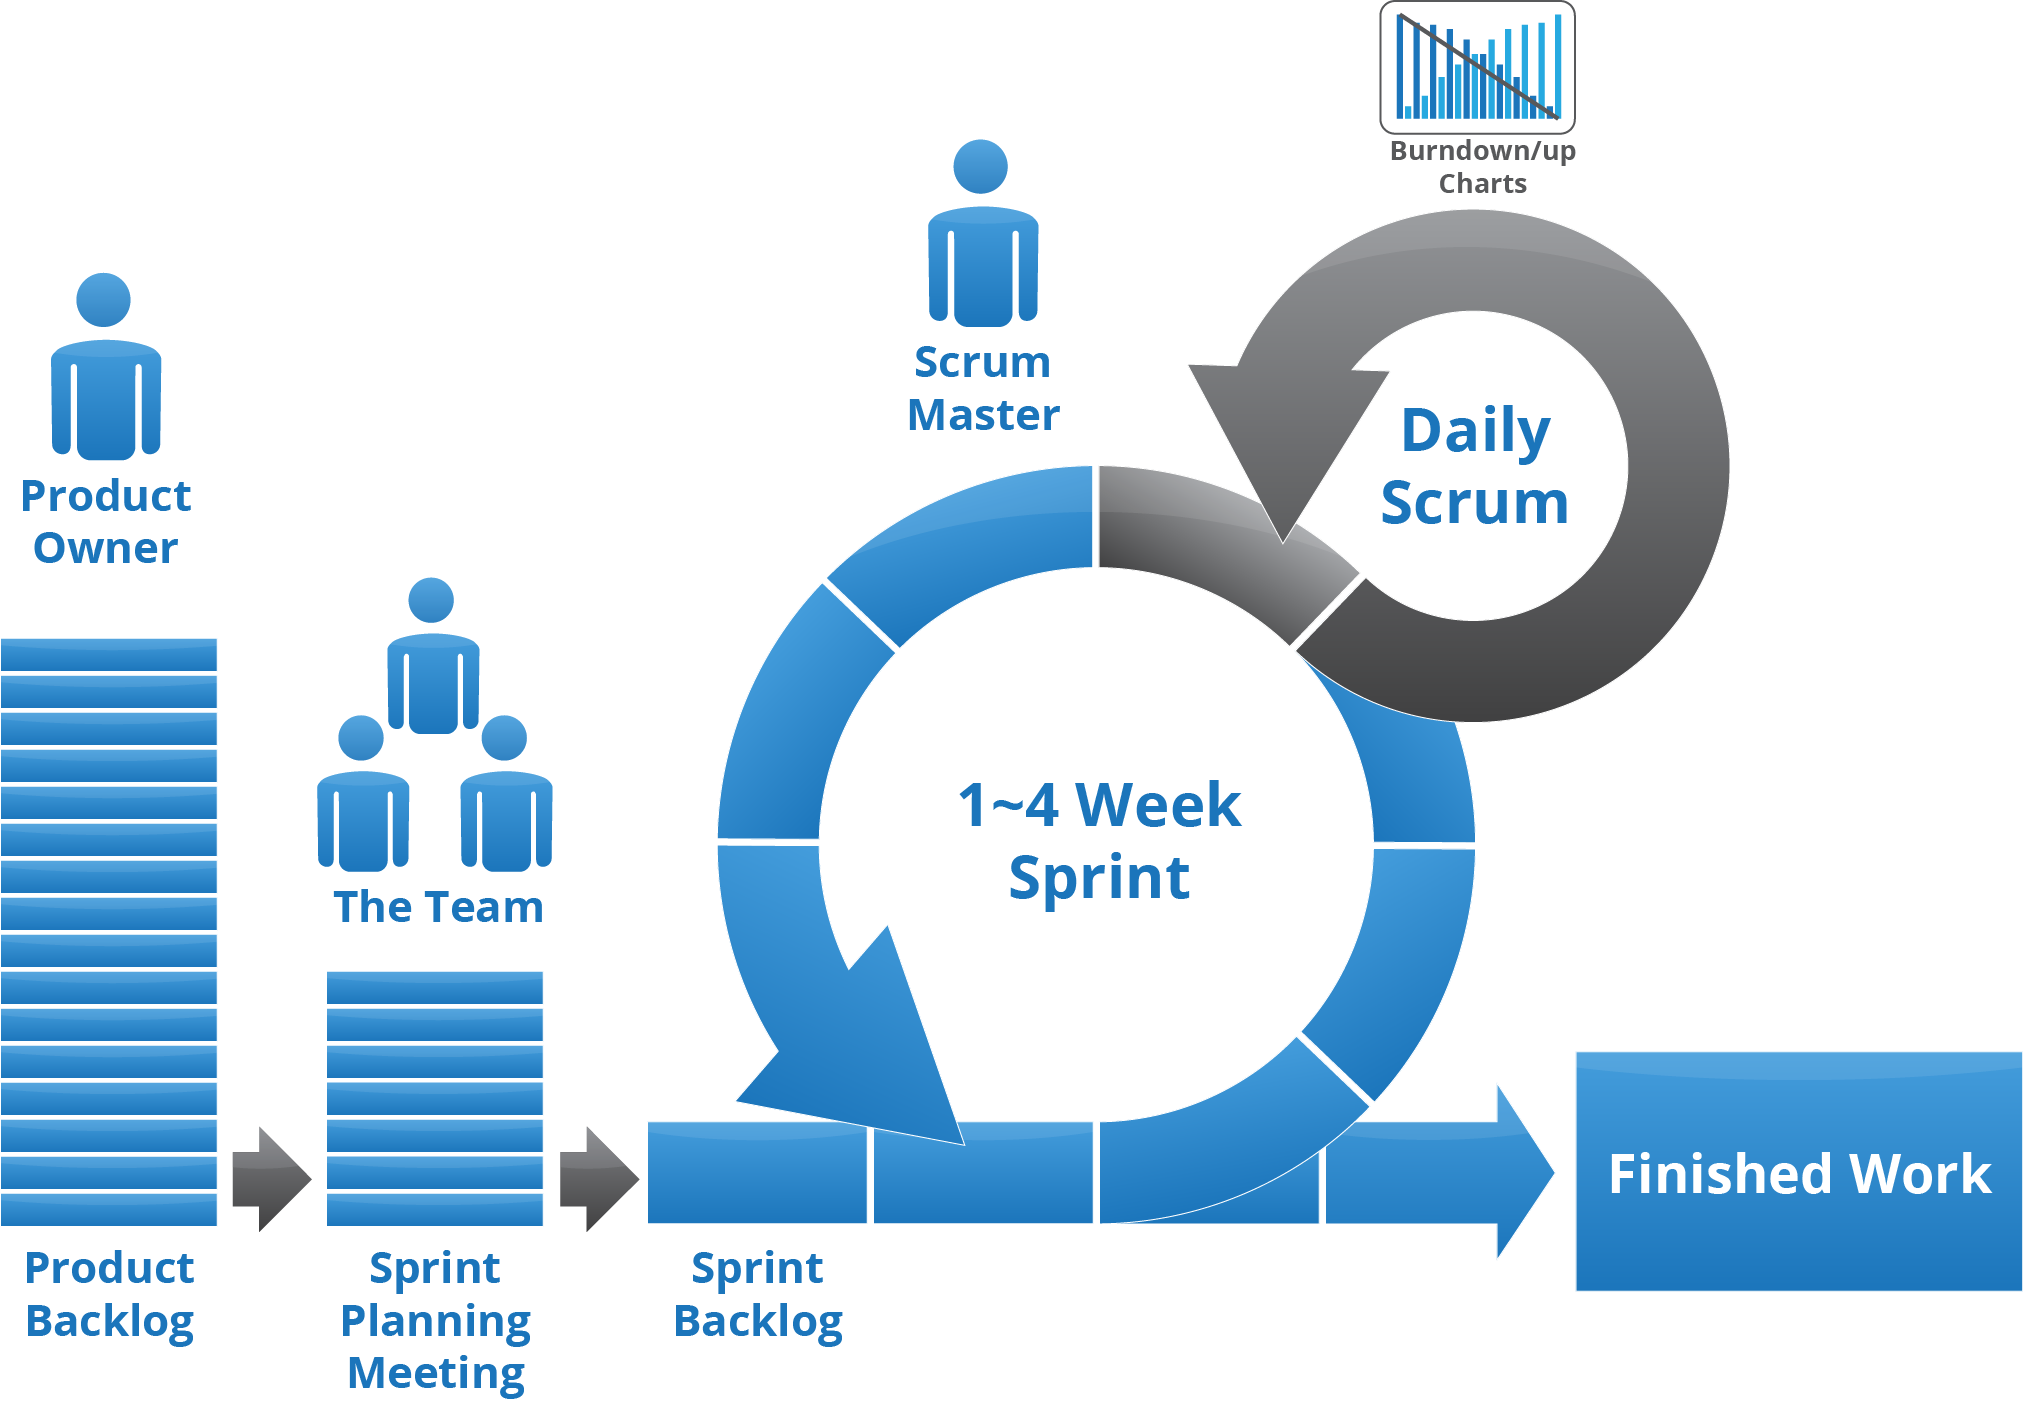
\includegraphics[scale=0.15]{images/scrum.png}
	\caption{The Scrum Process}\label{fig:scrum}
\end{figure}

\subsection{Theoretical Background}\label{scrum-theoretical-background}

\begin{flushleft}
	The original scrum guide is considered incomplete by its creators by design.
	Rather than defining detailed instructions to all teams worldwide, the rules
	of Scrum are intended to guide relationships and interactions between the people
	and their work. Founded on empiricism and lean thinking, Scrum asserts that
	knowledge comes from experience and making decisions based on what's observed.
	In a nutshell, it Scrum employs an iterative approach to optimize predictability
	and risk control. This methodology requires a cross-functional team working
	intensely together. Another positive side effect of this collaboration effort
	is that members of the team are encouraged to acquire and share knowledge together.
\end{flushleft}

\subsection{Transparency}\label{scrum-transparency}

\begin{flushleft}
	The emergent process and work must be visible to those performing the work
	as well as those receiving the work. With Scrum, important decisions are based
	on the perceived state of its three formal artifacts. Artifacts that have low
	transparency can lead to decisions that diminish value and increase risk.
	Transparency enables inspection. Inspection without transparency is misleading
	and wasteful.
\end{flushleft}

\subsection{Inspection}\label{scrum-inspection}

\begin{flushleft}
	The Scrum artifacts and the progress toward agreed goals must be inspected
	frequently and diligently to detect potentially undesirable variances or problems.
	To help with inspection, Scrum provides cadence in the form of its five events.
	Inspection enables adaptation. Inspection without adaptation is considered pointless.
	Scrum events are designed to provoke change.
\end{flushleft}

\subsection{Adaption}\label{scrum-adaption}

\begin{flushleft}
	If any aspects of a process deviate outside acceptable limits or if the resulting
	product is unacceptable, the process being applied or the materials being produced
	must be adjusted. The adjustment must be made as soon as possible to minimize
	further deviation. Adaptation becomes more difficult when the people involved are
	not empowered or self-managing. A Scrum Team is expected to adapt the moment it
	learns anything new through inspection.
\end{flushleft}

\subsection{Scrum Values}\label{scrum-values}

\begin{flushleft}
	Successful use of Scrum depends on people becoming more proficient in living five values:
\end{flushleft}

\begin{enumerate}
	\item Commitment
	\item Focus
	\item Openness
	\item Respect
	\item Courage
\end{enumerate}

\begin{flushleft}
	The primary focus of the Scrum team is on the work of the Sprints to make the
	best possible progress toward these goals. Both the team and the stakeholder
	are open about the work and the challenges involved. These value give direction
	to the Scrum Team with regard to their work, actions and behavior. Decisions
	being made should reinforce and not diminish these values; only when these
	values are embodied, the empirical Scrum pillars of transparency, inspection
	and adaption come to life building trust.
\end{flushleft}

\subsection{Scrum Team}\label{scrum-team}

\begin{flushleft}
	The Scrum team is fundamental to Scrum without it no work would get done.
	This team largely consists of three types of people whose roles are described
	in more detail in the subsections below. Ideally, you'd want to keep this
	team small enough to remain nimble and large enough to be able to complete the
	work within the designated time period. As a rule of thumb, 10 or fewer people
	make up such a team.
\end{flushleft}

\begin{flushleft}
	In the event that a team grows too much in size, consider reorganizing into
	multiple cohesive teams, each focused on the same product and sharing the same
	Product Goal, Product Backlog and Product Owner. The responsibilities that fall
	into the hand of the Scrum team includes:
\end{flushleft}

\begin{itemize}
	\item Product-related activities from stakeholder collaboration
	\item Verification
	\item Experimentation
	\item Research
	\item Development
	\item Anything else that might be required to meet the Product Goal
\end{itemize}

\begin{flushleft}
	Working in Sprints at a sustainable pace helps improve the team's focus and consistency.
\end{flushleft}

\subsection{Product Owner}\label{scrum-product-owner}

\begin{flushleft}
	The Product Owner (a single entity) is accountable for maximizing the value of
	the product resulting from the work of the Scrum Team. How this is done may vary
	widely across organizations, Scrum Teams, and individuals. They are also accountable
	for effective Product Backlog management, which includes:
\end{flushleft}

\begin{itemize}
	\item Developing and explicitly communicating the Product Goal
	\item Creating and clearly communicating the Product Backlog items
	\item Ordering Product Backlog items
	\item Ensuring that the Product Backlog is transparent, visible and understood
\end{itemize}

\begin{flushleft}
	The Product Owner may do the above work or may delegate the responsibility to
	others. Regardless, the Product Owner remains accountable. The Product Owner
	may represent the needs of many stakeholders in the Product Backlog. Those
	wanting to change the Product Backlog can do so by trying to convince the
	Product Owner because it's the product owner's responsibility to decide whether
	the software goes out at the end of a sprint. In short, the product owner is
	the gatekeeper for everything that comes in and goes out and thus may be
	considered a crucial point in the Scrum process, which is especially true
	from devsecops's points of view. However, it is also the product owner who's
	usually does not receive adequate security training.
\end{flushleft}

\subsection{Developers}\label{scrum-developers}

\begin{flushleft}
	Developers are the people in the Scrum Team that are committed to creating any
	aspect of a usable Increment each Sprint. The specific skills needed by the
	Developers are often broad and will vary with the domain of work. However, the
	Developers are always accountable for:
\end{flushleft}

\begin{itemize}
	\item Creating a plan for the Sprint, namely the Sprint Backlog
	\item Instilling quality by adhering to a Definition of Done
	\item Adapting their plan each day toward a Sprint Goal
	\item Holding each other accountable as professionals
\end{itemize}

\subsection{Scrum Master}\label{scrum-master}

\begin{flushleft}
	The Scrum Master is accountable for establishing Scrum as defined in the Scrum
	Guide. They do this by helping everyone understand Scrum theory and practice,
	both within the Scrum Team and the organization. The Scrum Master serves the
	Scrum Team in several ways, including:
\end{flushleft}

\begin{itemize}
	\item Coaching the team members in self-management and cross-functionality
	\item Helping the Scrum team focus on creating high-value Increments that meet the Definition of Done
	\item Causing the removal of impediments to the Scrum Team's progress
	\item Ensuring that all Scrum events take place and are positive, productive, and kept within the time box
\end{itemize}

\begin{flushleft}
	The Scrum Master serves the Product Owner in several ways, including:
\end{flushleft}

\begin{itemize}
	\item Helping find techniques for effective Product Goal definition and Product Backlog management
	\item Helping the Scrum Team understand the need for clear and concise Product Backlog items
	\item Helping establish empirical product planning for a complex environment
	\item Facilitating stakeholder collaboration as requested or needed
\end{itemize}

\begin{flushleft}
	The Scrum Master serves the organization in several ways, including:
\end{flushleft}

\begin{itemize}
	\item Leading, training, and coaching the organization in its Scrum adoption
	\item Planning and advising Scrum implementations within the organization
	\item Helping employees and stakeholders understand and enact an empirical approach for complex work
	\item Removing barriers between stakeholders and Scrum Teams
\end{itemize}

\subsection{Scrum Events}\label{scrum-events}

\begin{flushleft}
	The Sprint is a container for all other events. Each event in Scrum is a formal
	opportunity to inspect and adapt Scrum Artifacts. These events are specifically
	designed to enable the transparency required. Failure to operate any events as
	prescribed results in lost opportunities to inspect and adapt (see also: Scrum Values).
	Events are used in Scrum to create regularity and to minimize the need for meetings
	not defined in Scrum. Optimally, all events are held at the same time and place
	to reduce complexity.
\end{flushleft}

\subsection{Sprints}\label{scrum-sprints}

\begin{flushleft}
	Sprints are fixed length events of one month or less (typically two weeks in
	length) to create consistency. A new Sprint starts immediately after the conclusion
	of the previous Sprint. All the work necessary to achieve the Product Goal, including
	Sprint Planning, Daily Scrum, Sprint Review, and Sprint Retrospective, happen within
	Sprints. During the sprint no changes are made that would endanger the Sprint Goal,
	nor does the quality of the work decrease. Keep the backlog as refined as needed,
	and clarify and renegotiate the scope with the Product Owner as more is learned.
	Short sprints can be employed to generate more learning cycles and limit risk
	of cost and effort to a smaller time frame. At best, each sprint may be considered
	a small project itself. A sprint could be canceled if the Sprint Goal become
	obsolete, although only the Product Owner has the authority to cancel a sprint.
\end{flushleft}

\subsection{Sprint Planning}\label{scrum=srpint-planning}

\begin{flushleft}
	Sprint Planning initiates the Sprint by laying out the work to be performed
	for the Sprint. This resulting plan is created by the collaborative work of
	the entire Scrum Team. The Scrum Team may also invite other people to attend
	Sprint Planning to provide advice. Sprint Planning is timeboxed to a maximum
	of eight hours for a one-month Sprint. For shorter Sprints, the event is
	usually shorter. Sprint Planning addresses the following topics:
\end{flushleft}

\begin{flushleft}
	\textbf{Why is this Sprint valuable?} The Product Owner proposes how the product
	could increase its value and utility in the current Sprint. The whole Scrum Team
	then collaborates to define a Sprint Goal that communicates why the Sprint is
	valuable to stakeholders. The Sprint Goal must be finalized prior to the end of
	Sprint Planning.
\end{flushleft}

\begin{flushleft}
	\textbf{What can be Done this Sprint?} Through discussion with the Product Owner,
	the Developers select items from the Product Backlog to include in the current
	Sprint. The Scrum Team may refine these items during this process, which increases
	understanding and confidence. Selecting how much can be completed within a Sprint
	may be challenging. However, the more the Developers know about their past performance,
	their upcoming capacity, and their Definition of Done, the more confident they will
	be in their Sprint forecasts.
\end{flushleft}

\begin{flushleft}
	\textbf{How will the chosen work get done?} For each selected Product Backlog item,
	the Developers plan the work necessary to create an Increment that meets the Definition
	of Done. This is often done by decomposing Product Backlog items into smaller work
	items of one day or less. How this is done is at the sole discretion of the Developers.
	No one else tells them how to turn Product Backlog items into Increments of value.
	The Sprint Goal, the Product Backlog items selected for the Sprint, plus the plan
	for delivering them are together referred to as the Sprint Backlog.
\end{flushleft}

\subsection{Daily Scrum}\label{scrum-daily}

\begin{flushleft}
	The purpose of the Daily Scrum is to inspect progress toward the Sprint Goal and
	adapt the Sprint Backlog as necessary, adjusting the upcoming planned work. The
	Daily Scrum is a 15-minute event for the Developers of the Scrum Team. To reduce
	complexity, it is held at the same time and place every working day of the Sprint.
	If the Product Owner or Scrum Master are actively working on items in the
	Sprint Backlog, they participate as Developers. Daily Scrums improve communications,
	identify impediments, promote quick decision-making, and consequently eliminate the
	need for other meetings. The Daily Scrum is not the only time Developers are allowed
	to adjust their plan. They often meet throughout the day for more detailed discussions
	about adapting or re-planning the rest of the Sprint's work.
\end{flushleft}

\subsection{Sprint Review}\label{scrum-sprint-review}

\begin{flushleft}
	The purpose of the Sprint Review is to inspect the outcome of the Sprint and determine
	future adaptations. The Scrum Team presents the results of their work to key stakeholders
	and progress toward the Product Goal is discussed. During the event, the Scrum Team and
	stakeholders review what was accomplished in the Sprint and what has changed in their
	environment. Based on this information, attendees collaborate on what to do next. The
	Product Backlog may also be adjusted to meet new opportunities. The Sprint Review is
	a working session and the Scrum Team should avoid limiting it to a presentation. The
	Sprint Review is the second to last event of the Sprint and is timeboxed to a maximum
	of four hours for a one-month Sprint. For shorter Sprints, the event is usually shorter.
\end{flushleft}

\subsection{Sprint Retrospective}\label{scrum-sprint-retrospective}

\begin{flushleft}
	The purpose of the Sprint Retrospective is to plan ways to increase quality and
	effectiveness. The Scrum Team inspects how the last Sprints went with
	regards to individuals, interactions, processes, tools, and their Definition
	of Done. Inspected elements often vary with the domain of work. Assumptions
	that led them astray are identified and their origins explored. The Scrum Team
	discusses what went well during the Sprint, what problems it encountered, and
	how those problems were (or were not) solved. The Scrum Team identifies the most
	helpful changes to improve its effectiveness. The most impactful improvements are
	addressed as soon as possible. They may even be added to the Sprint Backlog for
	the next Sprint. The Sprint Retrospective concludes the Sprint. It is timeboxed
	to a maximum of three hours for a one-month Sprint. For shorter Sprints, the event
	is usually shorter.
\end{flushleft}

\subsection{Artifacts}\label{scrum-artifacts}

\begin{flushleft}
	Scrum's artifacts represent work or value. They are designed to maximize Transparency
	of key information. Thus, everyone inspecting them has the same basis for Adaption.
	Each artifact contains a commitment to ensure it provides information that enhances
	transparency and focus against which progress can be measured:
\end{flushleft}

\begin{itemize}
	\item For the Product Owner it is the Product Goal
	\item For the Sprint Backlog is is the Sprint Goal
	\item For the Increment it is the Definition of Done
\end{itemize}

\begin{flushleft}
	These commitments exist to reinforce empiricism and the Scrum values for the Scrum
	team and their stakeholders.
\end{flushleft}

\subsection{Product Backlog}\label{scrum-product-backlog}

\begin{flushleft}
	The Product Backlog is an emergent, ordered list of what is needed to improve
	the product. It is the single source of work undertaken by the Scrum Team. Product
	Backlog items that can be Done by the Scrum Team within one Sprint are deemed
	ready for selection in a Sprint Planning event. They usually acquire this degree
	of Transparency after refining activities. Product Backlog refinement is the act
	of breaking down and further defining Product Backlog items into smaller more
	precise items. This is an ongoing activity to add details, such as a description,
	order, and size. Attributes often vary with the domain of work. The Developers who
	will be doing the work are responsible for the sizing. The Product Owner may influence
	the Developers by helping them understand and select trade-offs.
\end{flushleft}

\subsection{Product Goal}\label{scrum-product-goal}

\begin{flushleft}
	The Product Goal describes a future state of the product which can serve as a target
	for the Scrum Team to plan against. The Product Goal is in the Product Backlog.
	The rest of the Product Backlog emerges to define ``what'' will fulfill the Product Goal.
\end{flushleft}

\begin{displaycquote}
	A product is a vehicle to deliver value. It has a clear boundary, known stakeholders,
	well-defined users or customers. A product could be a service, a physical product,
	or something more abstract.
\end{displaycquote}

\begin{flushleft}
	The Product Goal is the long-term objective for the Scrum Team. They must fulfill
	(or abandon) one objective before taking on the next.
\end{flushleft}

\subsection{Sprint Backlog}\label{scrum-sprint-backlog}

\begin{flushleft}
	The Sprint Backlog is composed of the Sprint Goal (why), the set of Product Backlog
	items selected for the Sprint (what), as well as an actionable plan for delivering
	the Increment (how). The Sprint Backlog is a plan by and for the Developers. It is
	a highly visible, real-time picture of the work that the Developers plan to accomplish
	during the Sprints in order to achieve the Sprint Goal. Consequently, the Sprint Backlog
	is updated throughout the Sprint as more is learned. It should have enough detail that
	they can inspect their progress in the Daily Scrum.
\end{flushleft}

\subsection{Increment}\label{scrum-increment}

\begin{flushleft}
	An Increment is a concrete stepping stone toward the Product Goal. Each Increment is
	additive to all prior Increments and thoroughly verified, ensuring that all Increments
	work together. In order to provide value, the Increment must be usable. Multiple
	Increments may be created within a Sprint. The sum of the Increments is presented at
	the Sprint Review thus supporting empiricism. However, an Increment may be delivered
	to stakeholders prior to the end of the Sprint. The Sprint Review should never be
	considered a gate to releasing value. Work cannot be considered part of an Increment
	unless it meets the Definition of Done.
\end{flushleft}

\subsection{Definition of Done}\label{scrum-definition-of-done}

\begin{flushleft}
	The Definition of Done is a formal description of the state of the Increment when
	it meets the quality measures required for the product. The moment a Product Backlog
	item meets the Definition of Done, an Increment is born. The Definition of Done
	creates Transparency by providing everyone a shared understanding of what work
	was completed as part of the Increment. If a Product Backlog item does not meet
	the Definition of Done, it cannot be released or even presented at the Sprint Review.
	Instead, it returns to the Product Backlog for future consideration. If the Definition
	of Done for an Increment is part of the standards of the organization, all Scrum Teams
	must follow it as a minimum. If it is not an organizational standard, the Scrum Team
	must create a Definition of Done appropriate for the product. The Developers are
	required to conform to the Definition of Done. If there are multiple Scrum Teams
	working together on a product, they must mutually define and comply with the same
	Definition of Done.
\end{flushleft}
